
\input{../../2021/style/preamble4tex}
% dependencies: amsmath, amssymb, dsfont
% math spaces
\ifdefined\N
\renewcommand{\N}{\mathds{N}} % N, naturals
\else \newcommand{\N}{\mathds{N}} \fi
\newcommand{\Z}{\mathds{Z}} % Z, integers
\newcommand{\Q}{\mathds{Q}} % Q, rationals
\newcommand{\R}{\mathds{R}} % R, reals
\ifdefined\C
\renewcommand{\C}{\mathds{C}} % C, complex
\else \newcommand{\C}{\mathds{C}} \fi
\newcommand{\continuous}{\mathcal{C}} % C, space of continuous functions
\newcommand{\M}{\mathcal{M}} % machine numbers
\newcommand{\epsm}{\epsilon_m} % maximum error

% counting / finite sets
\newcommand{\setzo}{\{0, 1\}} % set 0, 1
\newcommand{\setmp}{\{-1, +1\}} % set -1, 1
\newcommand{\unitint}{[0, 1]} % unit interval

% basic math stuff
\newcommand{\xt}{\tilde x} % x tilde
\DeclareMathOperator*{\argmax}{arg\,max} % argmax
\DeclareMathOperator*{\argmin}{arg\,min} % argmin
\newcommand{\argminlim}{\mathop{\mathrm{arg\,min}}\limits} % argmax with limits
\newcommand{\argmaxlim}{\mathop{\mathrm{arg\,max}}\limits} % argmin with limits
\newcommand{\sign}{\operatorname{sign}} % sign, signum
\newcommand{\I}{\mathbb{I}} % I, indicator
\newcommand{\order}{\mathcal{O}} % O, order
\newcommand{\bigO}{\mathcal{O}} % Big-O Landau
\newcommand{\littleo}{{o}} % Little-o Landau
\newcommand{\pd}[2]{\frac{\partial{#1}}{\partial #2}} % partial derivative
\newcommand{\floorlr}[1]{\left\lfloor #1 \right\rfloor} % floor
\newcommand{\ceillr}[1]{\left\lceil #1 \right\rceil} % ceiling
\newcommand{\indep}{\perp \!\!\! \perp} % independence symbol

% sums and products
\newcommand{\sumin}{\sum\limits_{i=1}^n} % summation from i=1 to n
\newcommand{\sumim}{\sum\limits_{i=1}^m} % summation from i=1 to m
\newcommand{\sumjn}{\sum\limits_{j=1}^n} % summation from j=1 to p
\newcommand{\sumjp}{\sum\limits_{j=1}^p} % summation from j=1 to p
\newcommand{\sumik}{\sum\limits_{i=1}^k} % summation from i=1 to k
\newcommand{\sumkg}{\sum\limits_{k=1}^g} % summation from k=1 to g
\newcommand{\sumjg}{\sum\limits_{j=1}^g} % summation from j=1 to g
\newcommand{\meanin}{\frac{1}{n} \sum\limits_{i=1}^n} % mean from i=1 to n
\newcommand{\meanim}{\frac{1}{m} \sum\limits_{i=1}^m} % mean from i=1 to n
\newcommand{\meankg}{\frac{1}{g} \sum\limits_{k=1}^g} % mean from k=1 to g
\newcommand{\prodin}{\prod\limits_{i=1}^n} % product from i=1 to n
\newcommand{\prodkg}{\prod\limits_{k=1}^g} % product from k=1 to g
\newcommand{\prodjp}{\prod\limits_{j=1}^p} % product from j=1 to p

% linear algebra
\newcommand{\one}{\bm{1}} % 1, unitvector
\newcommand{\zero}{\mathbf{0}} % 0-vector
\newcommand{\id}{\bm{I}} % I, identity
\newcommand{\diag}{\operatorname{diag}} % diag, diagonal
\newcommand{\trace}{\operatorname{tr}} % tr, trace
\newcommand{\spn}{\operatorname{span}} % span
\newcommand{\scp}[2]{\left\langle #1, #2 \right\rangle} % <.,.>, scalarproduct
\newcommand{\mat}[1]{\begin{pmatrix} #1 \end{pmatrix}} % short pmatrix command
\newcommand{\Amat}{\mathbf{A}} % matrix A
\newcommand{\Deltab}{\mathbf{\Delta}} % error term for vectors

% basic probability + stats
\renewcommand{\P}{\mathds{P}} % P, probability
\newcommand{\E}{\mathds{E}} % E, expectation
\newcommand{\var}{\mathsf{Var}} % Var, variance
\newcommand{\cov}{\mathsf{Cov}} % Cov, covariance
\newcommand{\corr}{\mathsf{Corr}} % Corr, correlation
\newcommand{\normal}{\mathcal{N}} % N of the normal distribution
\newcommand{\iid}{\overset{i.i.d}{\sim}} % dist with i.i.d superscript
\newcommand{\distas}[1]{\overset{#1}{\sim}} % ... is distributed as ...

% machine learning
\newcommand{\Xspace}{\mathcal{X}} % X, input space
\newcommand{\Yspace}{\mathcal{Y}} % Y, output space
\newcommand{\Zspace}{\mathcal{Z}} % Z, space of sampled datapoints
\newcommand{\nset}{\{1, \ldots, n\}} % set from 1 to n
\newcommand{\pset}{\{1, \ldots, p\}} % set from 1 to p
\newcommand{\gset}{\{1, \ldots, g\}} % set from 1 to g
\newcommand{\Pxy}{\mathbb{P}_{xy}} % P_xy
\newcommand{\Exy}{\mathbb{E}_{xy}} % E_xy: Expectation over random variables xy
\newcommand{\xv}{\mathbf{x}} % vector x (bold)
\newcommand{\xtil}{\tilde{\mathbf{x}}} % vector x-tilde (bold)
\newcommand{\yv}{\mathbf{y}} % vector y (bold)
\newcommand{\xy}{(\xv, y)} % observation (x, y)
\newcommand{\xvec}{\left(x_1, \ldots, x_p\right)^\top} % (x1, ..., xp)
\newcommand{\Xmat}{\mathbf{X}} % Design matrix
\newcommand{\allDatasets}{\mathds{D}} % The set of all datasets
\newcommand{\allDatasetsn}{\mathds{D}_n}  % The set of all datasets of size n
\newcommand{\D}{\mathcal{D}} % D, data
\newcommand{\Dn}{\D_n} % D_n, data of size n
\newcommand{\Dtrain}{\mathcal{D}_{\text{train}}} % D_train, training set
\newcommand{\Dtest}{\mathcal{D}_{\text{test}}} % D_test, test set
\newcommand{\xyi}[1][i]{\left(\xv^{(#1)}, y^{(#1)}\right)} % (x^i, y^i), i-th observation
\newcommand{\Dset}{\left( \xyi[1], \ldots, \xyi[n]\right)} % {(x1,y1)), ..., (xn,yn)}, data
\newcommand{\defAllDatasetsn}{(\Xspace \times \Yspace)^n} % Def. of the set of all datasets of size n
\newcommand{\defAllDatasets}{\bigcup_{n \in \N}(\Xspace \times \Yspace)^n} % Def. of the set of all datasets
\newcommand{\xdat}{\left\{ \xv^{(1)}, \ldots, \xv^{(n)}\right\}} % {x1, ..., xn}, input data
\newcommand{\ydat}{\left\{ \yv^{(1)}, \ldots, \yv^{(n)}\right\}} % {y1, ..., yn}, input data
\newcommand{\yvec}{\left(y^{(1)}, \hdots, y^{(n)}\right)^\top} % (y1, ..., yn), vector of outcomes
\newcommand{\greekxi}{\xi} % Greek letter xi
\renewcommand{\xi}[1][i]{\xv^{(#1)}} % x^i, i-th observed value of x
\newcommand{\yi}[1][i]{y^{(#1)}} % y^i, i-th observed value of y
\newcommand{\xivec}{\left(x^{(i)}_1, \ldots, x^{(i)}_p\right)^\top} % (x1^i, ..., xp^i), i-th observation vector
\newcommand{\xj}{\xv_j} % x_j, j-th feature
\newcommand{\xjvec}{\left(x^{(1)}_j, \ldots, x^{(n)}_j\right)^\top} % (x^1_j, ..., x^n_j), j-th feature vector
\newcommand{\phiv}{\mathbf{\phi}} % Basis transformation function phi
\newcommand{\phixi}{\mathbf{\phi}^{(i)}} % Basis transformation of xi: phi^i := phi(xi)

%%%%%% ml - models general
\newcommand{\lamv}{\bm{\lambda}} % lambda vector, hyperconfiguration vector
\newcommand{\Lam}{\bm{\Lambda}}	 % Lambda, space of all hpos
% Inducer / Inducing algorithm
\newcommand{\preimageInducer}{\left(\defAllDatasets\right)\times\Lam} % Set of all datasets times the hyperparameter space
\newcommand{\preimageInducerShort}{\allDatasets\times\Lam} % Set of all datasets times the hyperparameter space
% Inducer / Inducing algorithm
\newcommand{\ind}{\mathcal{I}} % Inducer, inducing algorithm, learning algorithm

% continuous prediction function f
\newcommand{\ftrue}{f_{\text{true}}}  % True underlying function (if a statistical model is assumed)
\newcommand{\ftruex}{\ftrue(\xv)} % True underlying function (if a statistical model is assumed)
\newcommand{\fx}{f(\xv)} % f(x), continuous prediction function
\newcommand{\fdomains}{f: \Xspace \rightarrow \R^g} % f with domain and co-domain
\newcommand{\Hspace}{\mathcal{H}} % hypothesis space where f is from
\newcommand{\fbayes}{f^{\ast}} % Bayes-optimal model
\newcommand{\fxbayes}{f^{\ast}(\xv)} % Bayes-optimal model
\newcommand{\fkx}[1][k]{f_{#1}(\xv)} % f_j(x), discriminant component function
\newcommand{\fh}{\hat{f}} % f hat, estimated prediction function
\newcommand{\fxh}{\fh(\xv)} % fhat(x)
\newcommand{\fxt}{f(\xv ~|~ \thetav)} % f(x | theta)
\newcommand{\fxi}{f\left(\xv^{(i)}\right)} % f(x^(i))
\newcommand{\fxih}{\hat{f}\left(\xv^{(i)}\right)} % f(x^(i))
\newcommand{\fxit}{f\left(\xv^{(i)} ~|~ \thetav\right)} % f(x^(i) | theta)
\newcommand{\fhD}{\fh_{\D}} % fhat_D, estimate of f based on D
\newcommand{\fhDtrain}{\fh_{\Dtrain}} % fhat_Dtrain, estimate of f based on D
\newcommand{\fhDnlam}{\fh_{\Dn, \lamv}} %model learned on Dn with hp lambda
\newcommand{\fhDlam}{\fh_{\D, \lamv}} %model learned on D with hp lambda
\newcommand{\fhDnlams}{\fh_{\Dn, \lamv^\ast}} %model learned on Dn with optimal hp lambda
\newcommand{\fhDlams}{\fh_{\D, \lamv^\ast}} %model learned on D with optimal hp lambda

% discrete prediction function h
\newcommand{\hx}{h(\xv)} % h(x), discrete prediction function
\newcommand{\hh}{\hat{h}} % h hat
\newcommand{\hxh}{\hat{h}(\xv)} % hhat(x)
\newcommand{\hxt}{h(\xv | \thetav)} % h(x | theta)
\newcommand{\hxi}{h\left(\xi\right)} % h(x^(i))
\newcommand{\hxit}{h\left(\xi ~|~ \thetav\right)} % h(x^(i) | theta)
\newcommand{\hbayes}{h^{\ast}} % Bayes-optimal classification model
\newcommand{\hxbayes}{h^{\ast}(\xv)} % Bayes-optimal classification model

% yhat
\newcommand{\yh}{\hat{y}} % yhat for prediction of target
\newcommand{\yih}{\hat{y}^{(i)}} % yhat^(i) for prediction of ith targiet
\newcommand{\resi}{\yi- \yih}

% theta
\newcommand{\thetah}{\hat{\theta}} % theta hat
\newcommand{\thetav}{\bm{\theta}} % theta vector
\newcommand{\thetavh}{\bm{\hat\theta}} % theta vector hat
\newcommand{\thetat}[1][t]{\thetav^{[#1]}} % theta^[t] in optimization
\newcommand{\thetatn}[1][t]{\thetav^{[#1 +1]}} % theta^[t+1] in optimization
\newcommand{\thetahDnlam}{\thetavh_{\Dn, \lamv}} %theta learned on Dn with hp lambda
\newcommand{\thetahDlam}{\thetavh_{\D, \lamv}} %theta learned on D with hp lambda
\newcommand{\mint}{\min_{\thetav \in \Theta}} % min problem theta
\newcommand{\argmint}{\argmin_{\thetav \in \Theta}} % argmin theta

% densities + probabilities
% pdf of x
\newcommand{\pdf}{p} % p
\newcommand{\pdfx}{p(\xv)} % p(x)
\newcommand{\pixt}{\pi(\xv~|~ \thetav)} % pi(x|theta), pdf of x given theta
\newcommand{\pixit}[1][i]{\pi\left(\xi[#1] ~|~ \thetav\right)} % pi(x^i|theta), pdf of x given theta
\newcommand{\pixii}[1][i]{\pi\left(\xi[#1]\right)} % pi(x^i), pdf of i-th x

% pdf of (x, y)
\newcommand{\pdfxy}{p(\xv,y)} % p(x, y)
\newcommand{\pdfxyt}{p(\xv, y ~|~ \thetav)} % p(x, y | theta)
\newcommand{\pdfxyit}{p\left(\xi, \yi ~|~ \thetav\right)} % p(x^(i), y^(i) | theta)

% pdf of x given y
\newcommand{\pdfxyk}[1][k]{p(\xv | y= #1)} % p(x | y = k)
\newcommand{\lpdfxyk}[1][k]{\log p(\xv | y= #1)} % log p(x | y = k)
\newcommand{\pdfxiyk}[1][k]{p\left(\xi | y= #1 \right)} % p(x^i | y = k)

% prior probabilities
\newcommand{\pik}[1][k]{\pi_{#1}} % pi_k, prior
\newcommand{\lpik}[1][k]{\log \pi_{#1}} % log pi_k, log of the prior
\newcommand{\pit}{\pi(\thetav)} % Prior probability of parameter theta

% posterior probabilities
\newcommand{\post}{\P(y = 1 ~|~ \xv)} % P(y = 1 | x), post. prob for y=1
\newcommand{\postk}[1][k]{\P(y = #1 ~|~ \xv)} % P(y = k | y), post. prob for y=k
\newcommand{\pidomains}{\pi: \Xspace \rightarrow \unitint} % pi with domain and co-domain
\newcommand{\pibayes}{\pi^{\ast}} % Bayes-optimal classification model
\newcommand{\pixbayes}{\pi^{\ast}(\xv)} % Bayes-optimal classification model
\newcommand{\pix}{\pi(\xv)} % pi(x), P(y = 1 | x)
\newcommand{\piv}{\bm{\pi}} % pi, bold, as vector
\newcommand{\pikx}[1][k]{\pi_{#1}(\xv)} % pi_k(x), P(y = k | x)
\newcommand{\pikxt}[1][k]{\pi_{#1}(\xv ~|~ \thetav)} % pi_k(x | theta), P(y = k | x, theta)
\newcommand{\pixh}{\hat \pi(\xv)} % pi(x) hat, P(y = 1 | x) hat
\newcommand{\pikxh}[1][k]{\hat \pi_{#1}(\xv)} % pi_k(x) hat, P(y = k | x) hat
\newcommand{\pixih}{\hat \pi(\xi)} % pi(x^(i)) with hat
\newcommand{\pikxih}[1][k]{\hat \pi_{#1}(\xi)} % pi_k(x^(i)) with hat
\newcommand{\pdfygxt}{p(y ~|~\xv, \thetav)} % p(y | x, theta)
\newcommand{\pdfyigxit}{p\left(\yi ~|~\xi, \thetav\right)} % p(y^i |x^i, theta)
\newcommand{\lpdfygxt}{\log \pdfygxt } % log p(y | x, theta)
\newcommand{\lpdfyigxit}{\log \pdfyigxit} % log p(y^i |x^i, theta)

% probababilistic
\newcommand{\bayesrulek}[1][k]{\frac{\P(\xv | y= #1) \P(y= #1)}{\P(\xv)}} % Bayes rule
\newcommand{\muk}{\bm{\mu_k}} % mean vector of class-k Gaussian (discr analysis)

% residual and margin
\newcommand{\eps}{\epsilon} % residual, stochastic
\newcommand{\epsv}{\bm{\epsilon}} % residual, stochastic, as vector
\newcommand{\epsi}{\epsilon^{(i)}} % epsilon^i, residual, stochastic
\newcommand{\epsh}{\hat{\epsilon}} % residual, estimated
\newcommand{\epsvh}{\hat{\epsv}} % residual, estimated, vector
\newcommand{\yf}{y \fx} % y f(x), margin
\newcommand{\yfi}{\yi \fxi} % y^i f(x^i), margin
\newcommand{\Sigmah}{\hat \Sigma} % estimated covariance matrix
\newcommand{\Sigmahj}{\hat \Sigma_j} % estimated covariance matrix for the j-th class

% ml - loss, risk, likelihood
\newcommand{\Lyf}{L\left(y, f\right)} % L(y, f), loss function
\newcommand{\Lypi}{L\left(y, \pi\right)} % L(y, pi), loss function
\newcommand{\Lxy}{L\left(y, \fx\right)} % L(y, f(x)), loss function
\newcommand{\Lxyi}{L\left(\yi, \fxi\right)} % loss of observation
\newcommand{\Lxyt}{L\left(y, \fxt\right)} % loss with f parameterized
\newcommand{\Lxyit}{L\left(\yi, \fxit\right)} % loss of observation with f parameterized
\newcommand{\Lxym}{L\left(\yi, f\left(\bm{\tilde{x}}^{(i)} ~|~ \thetav\right)\right)} % loss of observation with f parameterized
\newcommand{\Lpixy}{L\left(y, \pix\right)} % loss in classification
\newcommand{\Lpiv}{L\left(y, \piv\right)} % loss in classification
\newcommand{\Lpixyi}{L\left(\yi, \pixii\right)} % loss of observation in classification
\newcommand{\Lpixyt}{L\left(y, \pixt\right)} % loss with pi parameterized
\newcommand{\Lpixyit}{L\left(\yi, \pixit\right)} % loss of observation with pi parameterized
\newcommand{\Lhxy}{L\left(y, \hx\right)} % L(y, h(x)), loss function on discrete classes
\newcommand{\Lr}{L\left(r\right)} % L(r), loss defined on residual (reg) / margin (classif)
\newcommand{\lone}{|y - \fx|} % L1 loss
\newcommand{\ltwo}{\left(y - \fx\right)^2} % L2 loss
\newcommand{\lbernoullimp}{\ln(1 + \exp(-y \cdot \fx))} % Bernoulli loss for -1, +1 encoding
\newcommand{\lbernoullizo}{- y \cdot \fx + \log(1 + \exp(\fx))} % Bernoulli loss for 0, 1 encoding
\newcommand{\lcrossent}{- y \log \left(\pix\right) - (1 - y) \log \left(1 - \pix\right)} % cross-entropy loss
\newcommand{\lbrier}{\left(\pix - y \right)^2} % Brier score
\newcommand{\risk}{\mathcal{R}} % R, risk
\newcommand{\riskbayes}{\mathcal{R}^\ast}
\newcommand{\riskf}{\risk(f)} % R(f), risk
\newcommand{\riskdef}{\E_{y|\xv}\left(\Lxy \right)} % risk def (expected loss)
\newcommand{\riskt}{\mathcal{R}(\thetav)} % R(theta), risk
\newcommand{\riske}{\mathcal{R}_{\text{emp}}} % R_emp, empirical risk w/o factor 1 / n
\newcommand{\riskeb}{\bar{\mathcal{R}}_{\text{emp}}} % R_emp, empirical risk w/ factor 1 / n
\newcommand{\riskef}{\riske(f)} % R_emp(f)
\newcommand{\risket}{\mathcal{R}_{\text{emp}}(\thetav)} % R_emp(theta)
\newcommand{\riskr}{\mathcal{R}_{\text{reg}}} % R_reg, regularized risk
\newcommand{\riskrt}{\mathcal{R}_{\text{reg}}(\thetav)} % R_reg(theta)
\newcommand{\riskrf}{\riskr(f)} % R_reg(f)
\newcommand{\riskrth}{\hat{\mathcal{R}}_{\text{reg}}(\thetav)} % hat R_reg(theta)
\newcommand{\risketh}{\hat{\mathcal{R}}_{\text{emp}}(\thetav)} % hat R_emp(theta)
\newcommand{\LL}{\mathcal{L}} % L, likelihood
\newcommand{\LLt}{\mathcal{L}(\thetav)} % L(theta), likelihood
\newcommand{\LLtx}{\mathcal{L}(\thetav | \xv)} % L(theta|x), likelihood
\newcommand{\logl}{\ell} % l, log-likelihood
\newcommand{\loglt}{\logl(\thetav)} % l(theta), log-likelihood
\newcommand{\logltx}{\logl(\thetav | \xv)} % l(theta|x), log-likelihood
\newcommand{\errtrain}{\text{err}_{\text{train}}} % training error
\newcommand{\errtest}{\text{err}_{\text{test}}} % test error
\newcommand{\errexp}{\overline{\text{err}_{\text{test}}}} % avg training error

% lm
\newcommand{\thx}{\thetav^\top \xv} % linear model
\newcommand{\olsest}{(\Xmat^\top \Xmat)^{-1} \Xmat^\top \yv} % OLS estimator in LM

\input{../../latex-math/ml-bagging.tex}
\input{../../latex-math/ml-boosting.tex}
% ml - trees, extra trees

\newcommand{\Np}{\mathcal{N}} % (Parent) node N
\newcommand{\Npk}{\Np_k} % node N_k
\newcommand{\Nl}{\Np_1}	% Left node N_1
\newcommand{\Nr}{\Np_2} % Right node N_2
\newcommand{\pikN}[1][k]{\pi_#1^{(\Np)}} % class probability node N
\newcommand{\pikNh}[1][k]{\hat\pi_#1^{(\Np)}} % estimated class probability node N
\newcommand{\pikNlh}[1][k]{\hat\pi_#1^{(\Nl)}} % estimated class probability left node
\newcommand{\pikNrh}[1][k]{\hat\pi_#1^{(\Nr)}} % estimated class probability right node


\begin{document}

\lecturechapter{11}{Gradient Boosting for Classification}
\lecture{Fortgeschrittene Computerintensive Methoden}


\begin{vbframe}{Binary classification}


For $\Yspace = \{0, 1\}$, we simply have to select an appropriate loss function, so let us
use Bernoulli loss as in logistic regression:

$$ \Lxy = - y \cdot \fx + \log(1 + \exp(\fx)).$$

Then,

\vspace{-0.5cm}

\begin{align*}
\tilde{r} &=-\fp{\Lxy}{\fx} \\
&= y - \frac{\exp(\fx)}{1 + \exp(\fx)} \\
&= y - \frac{1}{1 + \exp(-\fx)} = y - s(\fx).
\end{align*}

Here, $s(\fx)$ is the logistic function, applied to a scoring model.
Hence, effectively, the pseudo-residuals are $y - \pix$.

Through $\pix = s(\fx)$ we can also estimate posterior probabilities.

\framebreak
%

\begin{itemize}
\item Using this loss function, we can simply run GB as for regression.
  NB: Also here, we fit regression base learners against our numerical 
  vector of pseudo-residuals with L2 loss. 
\item The tree extension for boosting for the binary case works exactly as in regression.
\item  We could also have used the exponential loss for classification with 
  GB. It can be shown that the resulting GB algorithm is basically equivalent 
    to AdaBoost. In practice there is no big difference, although Bernoulli loss 
    makes a bit more sense from a theoretical (maximum likelihood) perspective.
\item It follows that GB is a generalization of AdaBoost which can also use other loss functions and be used for different ML scenarios.
\end{itemize}


\end{vbframe}



% \section{Interactive Playgrounds}
% 
% \begin{vbframe}{Gradient Boosting Playground}
% \begin{center}
% 
% 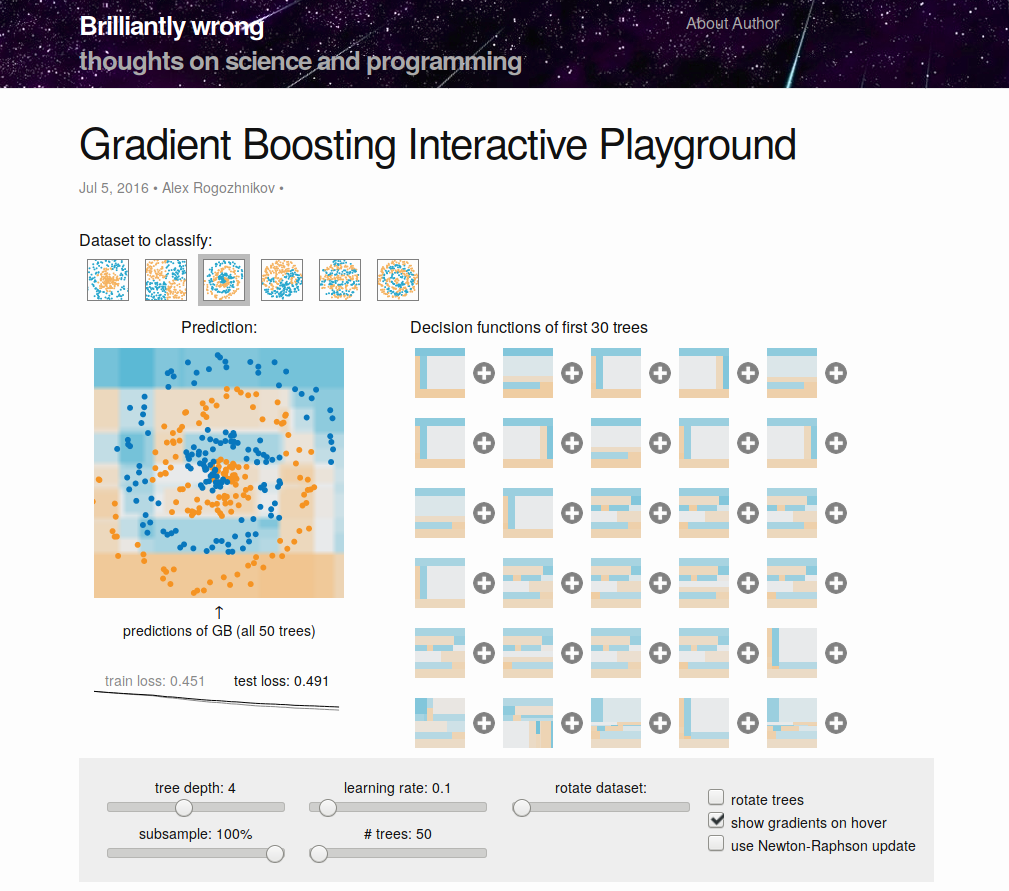
\includegraphics[width=0.7\textwidth]{figure_man/gbm_playground.png}
% 
% \href{http://arogozhnikov.github.io/2016/07/05/gradient_boosting_playground.html}{\beamergotobutton{Open in browser.}}
% 
% \end{center}
% \end{vbframe}
% 
% \begin{vbframe}{mlrPlayground}
% \begin{center}
% 
% 
\includegraphics[width=\linewidth]{figure_man/mlrplayground_welcome.png}
% 
% \href{https://compstat-lmu.shinyapps.io/mlrPlayground/}{\beamergotobutton{Open in browser.}}
% 
% \end{center}
% \end{vbframe}

% \section{Gradient Boosting for Multiclass Problems}

\begin{vbframe}{Multiclass problems}

We proceed as in softmax regression and model a categorical distribution with multinomial / log loss.
For $\Yspace = \{1, \ldots, g\}$, we create $g$ discriminant functions $\fxk$, one for each class and each one being an \textbf{additive} model of base learners.

We define the $\pi_k(\xv)$ through the softmax function:
$$ \pikx = s_k(f_1(\xv), \ldots, f_g(\xv)) = \exp(\fxk) / \sum_{j=1}^g \exp(f_j(\xv)). $$

Multinomial loss $L$:
$$ L(y, f_1(\xv), \ldots f_g(\xv)) = - \sumkg \mathds{1}_{\{y = k\}} \ln \pikx. $$

Pseudo-residuals:
$$-\fp{L(y, f_1(\xv), \ldots, f_g(\xv))}{\fxk} =  \mathds{1}_{\{y = k\}} - \pikx. $$


\framebreak

\begin{algorithm}[H]
  \begin{footnotesize}
  \begin{center}
  \caption{GB for Multiclass}
    \begin{algorithmic}[1]
      \State Initialize $f_{k}^{[0]}(\xv) = 0,\ k = 1,\ldots,g$
      \For{$m = 1 \to M$}
      \State Set $\pik^{[m]}(\xv) = \frac{\exp(f_k^{[m]}(\xv))}{\sum_j \exp(f_j^{[m]}(\xv))}, k = 1,\ldots,g$
            \For{$k = 1 \to g$}
            \State For all $i$: Compute $\rmi_k = \mathds{1}_{\{\yi = k\}} - \pik^{[m]}(\xi)$
              \State Fit a regression base learner $\hat{b}^{[m]}_k$ to the pseudo-residuals $\rmi_k$.
              \State Obtain $\betamh_k$ by constant learning rate or line-search.
              \State Update $\hat{f}_k^{[m]} = \hat{f}_k^{[m-1]} + \betamh_k \hat{b}^{[m]}_k$
            \EndFor
      \EndFor
    \State Output $\hat{f}_1^{[M]}, \ldots, \hat{f}_g^{[M]}$
    \end{algorithmic}
    \end{center}
    \end{footnotesize}
\end{algorithm}

\end{vbframe}

\begin{vbframe}{GB Multiclass with Trees}

\begin{itemize}
  \item From Friedman, J. H. - Greedy Function Approximation: A Gradient Boosting Machine (1999)
  \item Determining the tree structure for each $\hat{b}^{[m]}_k$ by L2 loss works just like before in the 2-class problem.
\item In the estimation of the $c$ values, so the heights of the terminal regions, however, all models depend on each other because of the definition
of $L$. Optimizing this is more difficult, so we will skip some details and present the main idea and results.
\end{itemize}

\framebreak

\begin{itemize}
  \item The post-hoc, loss optimal heights of the terminals $\hat{c}_{tk}^{[m]}$ are:
  $$ 
  \hat{c}_{tk}^{[m]} = - \argmin_{c_{tk}^{[m]} } \sum_{i=1}^n \sum_{k=1}^g \mathds{1}_{\{y = k\}} \ln \pi_k^{[m]}(\xv^{(i)}) \,,
  $$
\item Softmax trafo: $\pi_k^{[m]}(\xv) = \frac{\exp(f_k^{[m]}(\xv))}{\sum_j \exp(f_j^{[m]}(\xv))},$ with 
\item The k-th model:
  $
  \hat{f}_k^{[m]}(\xv^{(i)})) = \hat{f}_k^{[m-1]}(\xv^{(i)}) + \sum_{t=1}^{T_k^{[m]}} \hat{c}_{tk}^{[m]} \mathds{1}_{\{\xv^{(i)} \in R_{tk}^{[m]}\}} 
  $
  % resulting from the multinomial loss function $L(y, f_1(\xv), \ldots f_g(\xv)) = - \sumkg \mathds{1}_{\{y = k\}} \ln \pikx$.
  %and $\pikx = \frac{\exp(f_k(\xv))}{\sum_j \exp(f_j(\xv))}$ as before.\medskip

\end{itemize}


  % \item In each iteration $m$ we calculate the pseudo-residuals
        % $$\rmi_k = \mathds{1}_{\{\yi = k\}} - \pi_k^{[m-1]}(\xi),$$
        % where $\pi_k^{[m-1]}(\xi)$ is derived from $f^{[m-1]}(\mathbf{x}).$

  % \item Thus, $g$ trees are induced at each iteration $m$ to predict the corresponding current pseudo-residuals for each class on the probability scale.

  % \item Each of these trees has $T$ terminal nodes with corresponding regions $R_{tk}^{[m]}$.


\framebreak


\begin{itemize}

  \item There is no closed-form solution for finding the optimal $\hat{c}_{tk}^{[m]}$ values. Additionally, the regions corresponding to the different class trees overlap, so that the solution does not reduce to a separate calculation within each region of each tree.

  \item Hence, we approximate the solution with a single Newton-Raphson step, using a diagonal approximation to the Hessian (we leave out the details here).

  \item This decomposes the problem into a separate calculation for each terminal node of each tree.

  \item The result is

  $$\hat{c}_{tk}^{[m]} =
      \frac{g-1}{g}\frac{\sum_{\xi \in R_{tk}^{[m]}} \rmi_k}{\sum_{\xi \in R_{tk}^{[m]}} \left|\rmi_k\right|\left(1 - \left|\rmi_k\right|\right)}.$$

  % \item The update is then done by
  % $$
  % \hat{f}_k^{[m]}(\xv) = \hat{f}_k^{[m-1]}(\xv) + \sum_t \hat{c}_{tk}^{[m]} \mathds{1}_{\{\xv \in R_{tk}^{[m]}\}}.
  % $$

\end{itemize}

\framebreak


\begin{algorithm}[H]
  \begin{footnotesize}
  \begin{center}
  \caption{Gradient Boosting for $K$-class Classification.}
    \begin{algorithmic}[1]
      \State Initialize $f_{k}^{[0]}(\xb) = 0,\ k = 1,\ldots,g$
      \For{$m = 1 \to M$}
          \State Set $\pikx = \frac{\exp(f_k(x))}{\sum_j \exp(f_j(x))}, k = 1,\ldots,g$
            \For{$k = 1 \to g$}
              \State For all $i$: Compute $\rmi_k = \I(\yi = k) - \pi_k(\xi)$
              \State Fit regr. tree to the $\rmi_k$ giving terminal regions $R_{tk}^{[m]}$
              \State Compute
              \State \hskip\algorithmicindent\relax $\hat{c}_{tk}^{[m]} =
                \frac{g-1}{g}\frac{\sum_{\xi \in R_{tk}^{[m]}} \rmi_k}{\sum_{\xi \in R_{tk}^{[m]}} \left|\rmi_k\right|\left(1 - \left|\rmi_k\right|\right)}$
              \State Update $\hat{f}_k^{[m]}(\xb) = \hat{f}_k^{[m-1]}(x) + \sum_t \hat{c}_{tk}^{[m]} \I\left(x \in R_{tk}^{[m]}\right)$
            \EndFor
      \EndFor
    \State Output $\hat{f}_1^{[M]}, \ldots, \hat{f}_g^{[M]}$
    \end{algorithmic}
    \end{center}
    \end{footnotesize}
\end{algorithm}



\end{vbframe}


% \begin{vbframe}{Additional information}
% 
% By choosing a suitable loss function it is also possible to model a large number of different problem domains:
% \begin{itemize}
%   \item Regression
%   \item (Multiclass) Classification
%   \item Count data
%   \item Survival data
%   \item Ordinal data
%   \item Quantile regression
%   \item Ranking problems
%   \item ...
% \end{itemize}
% 
% \lz
% 
% % Boosting is closely related to L1 regularization.
% 
% % \lz
% 
% Different base learners increase flexibility (see componentwise gradient boosting).
% If we model only individual variables, the resulting regularized variable selection
% is closely related to $L1$ regularization.
% 
% \framebreak
% 
% For example, using the pinball loss in boosting
% $$
% L(y, f(\xv)) = \left\{
% \begin{array}{lc}
% (1 - \alpha)(f(\xv) - y), & \text{if}\ y < f(\xv) \\
% \alpha(y - f(\xv)),       & \text{if}\ y \geq f(\xv)
% \end{array}
% \right.
% $$
% models the $\alpha$-quantiles:
% 
% \begin{center}
% 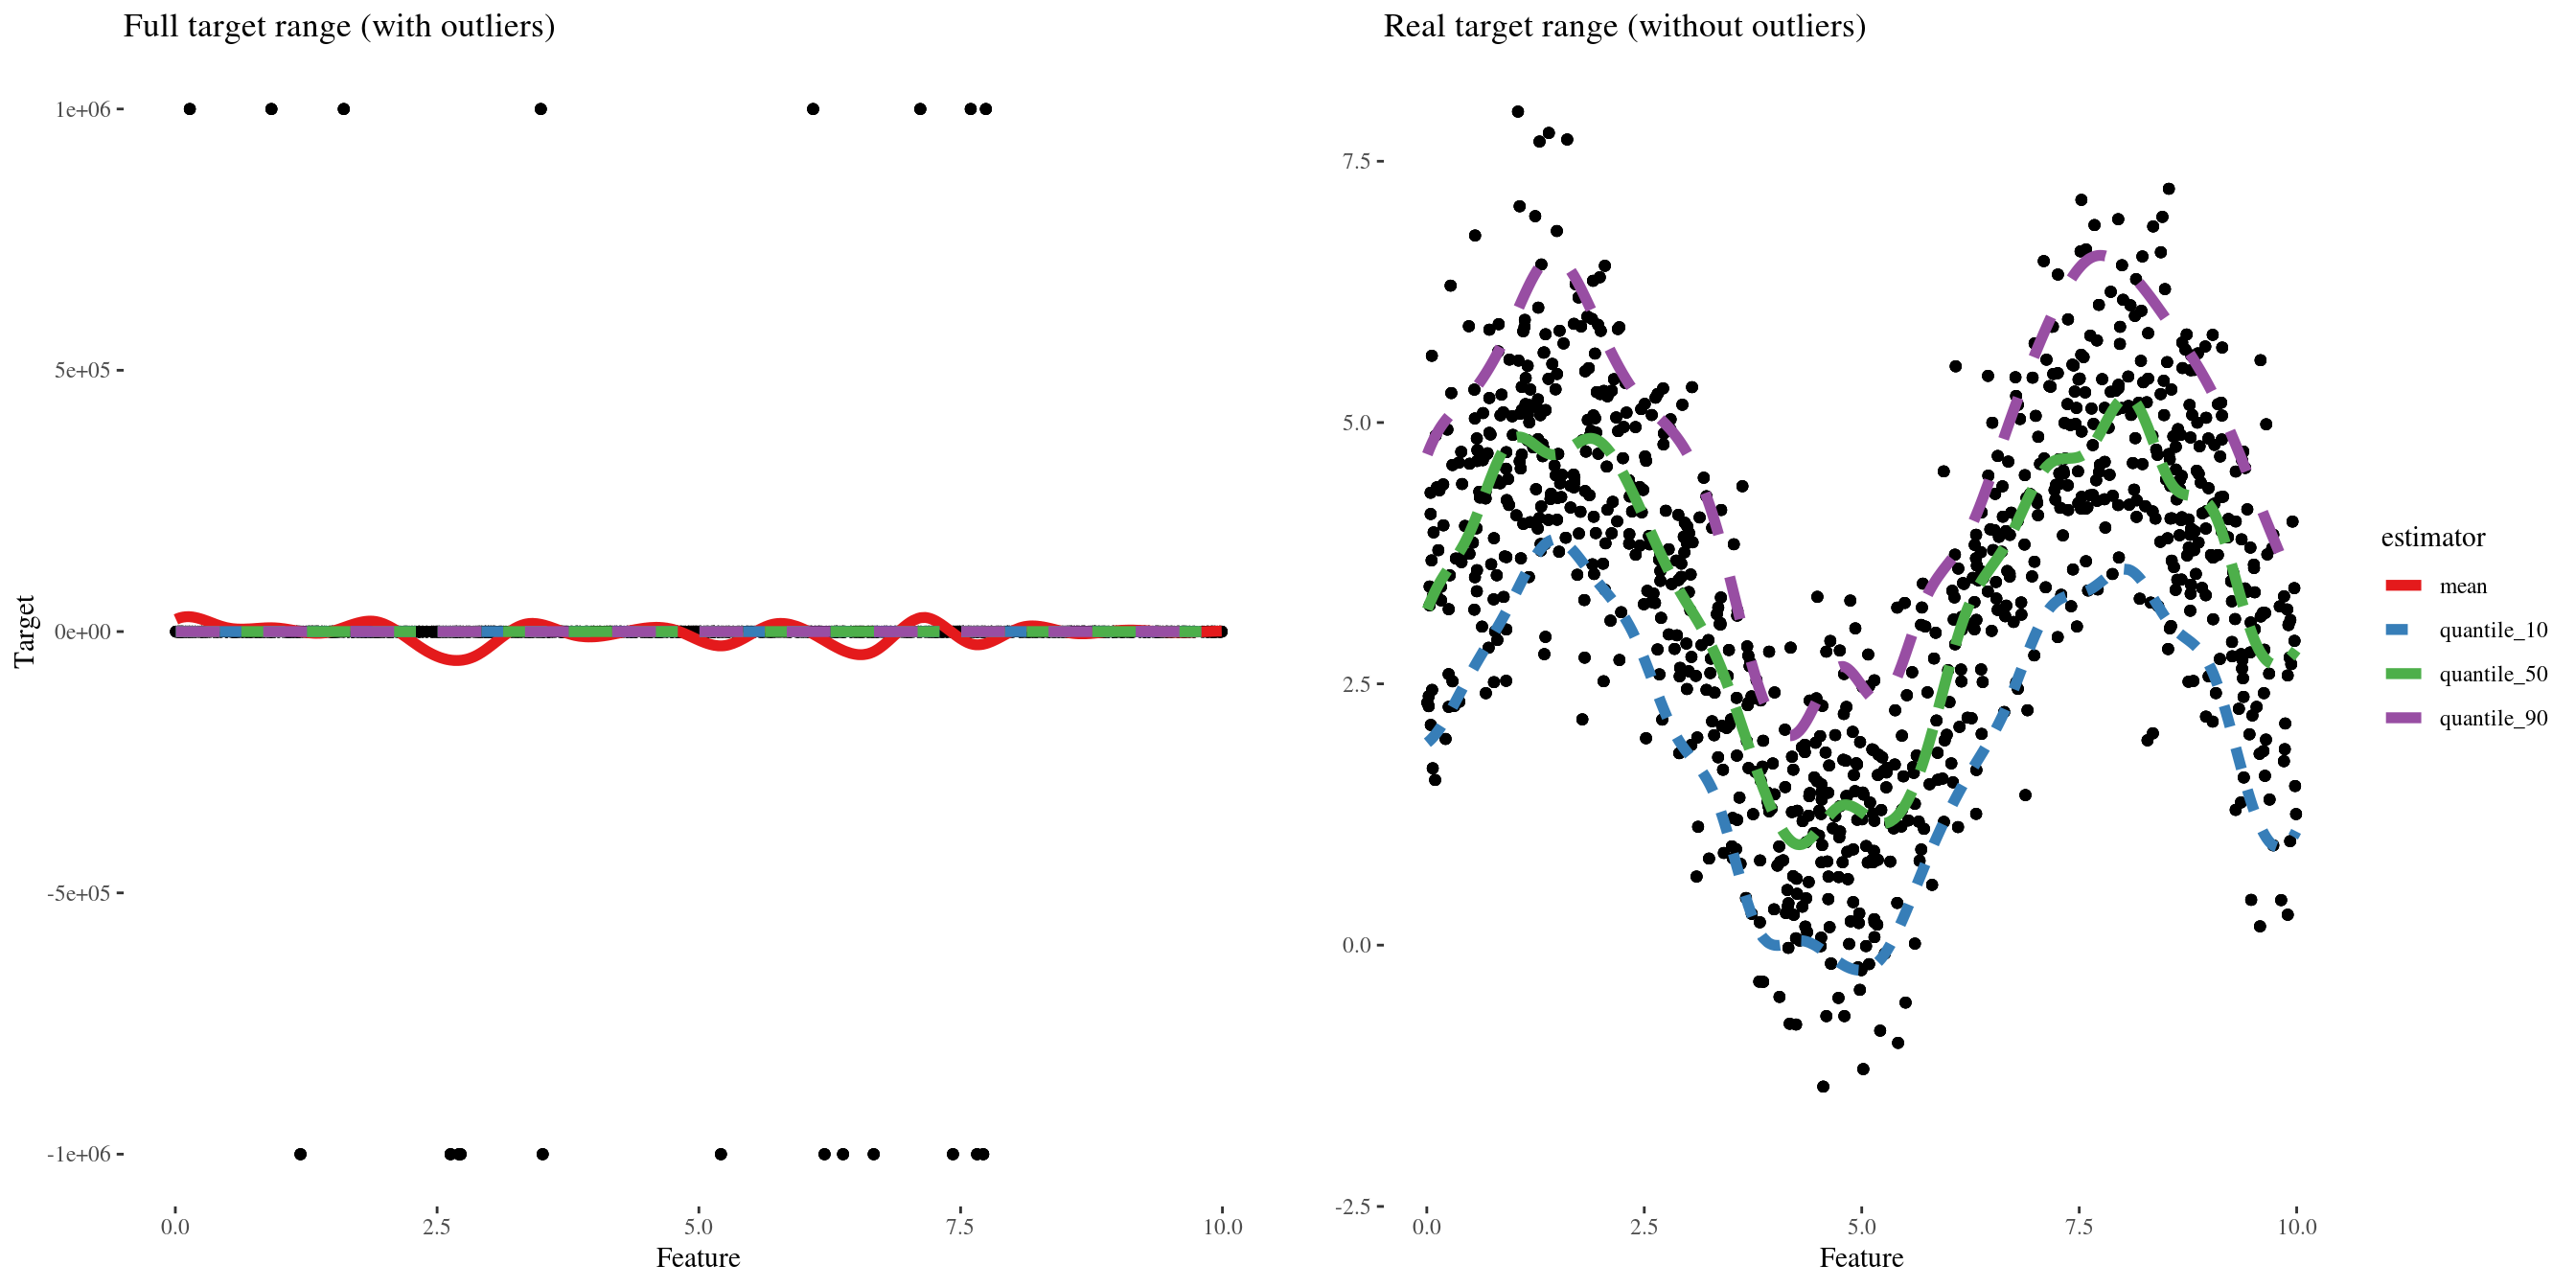
\includegraphics[scale=0.5]{figure_man/quantile_boosting.png}
% \end{center}
% 
% \framebreak
% 
% The AdaBoost fit has the structure of an additive model with \enquote{basis functions} $\bmm (x)$.
% 
% \lz
% 
% It can be shown (see Hastie et al. 2009, Chapter 10) that AdaBoost corresponds to minimizing the empirical risk in each iteration $m$ using the \textbf{exponential} loss function:
% \begin{align*}
%   L(y, \fmh(\mathbf{x}))    &= \exp\left(-y\fmh(\mathbf{x})\right) \\
%   \riske(\fmh)              &= \sumin L(\yi, \fmh(\xi)) \\
%                             &= \sumin L(\yi, \fmdh(\xi) + \beta b(\xi))\,,
% \end{align*}
% 
% 
% % \begin{align*}
% %   \sum_{i=1}^n \exp\left(-\yi \cdot \left(\beta b\left(\xi\right)
% %   + \fmdh\left(\xi\right)\right)\right),
% % \end{align*}
% with minimization over $\beta$ and $b$ and where $\fmdh$ is the boosting fit in iteration $m-1$.
% 
% % \framebreak
% 
% % AdaBoost is the empirical equivalent to the forward piecewise solution of the minimization problem
% 
% % \begin{align*}
% %   \text{arg} \min_{f} \E_{y|x}( \exp (- y \cdot \fx))\ .
% % \end{align*}
% 
% % \lz
% 
% % Therefore, the boosting fit is an estimate of function
% % \begin{align*}
% %   f^*(x) = 0.5 \cdot \log \left( \frac{\text{P} (y = 1 | x)}
% %   {\text{P} (y = -1 | x)}\right) \ ,
% % \end{align*}
% % which solves the former problem theoretically.
% 
% % \lz
% 
% % Obvious idea: generalization on other loss functions, use of alternative basis methods.
% 
% \end{vbframe}

% 
% \begin{vbframe}{Take home message}
% Gradient boosting is a statistical reinterpretation of the older AdaBoost algorithm.
% 
% \lz
% 
% Base learners are added in a \enquote{greedy} fashion, so that they point in the direction of the negative gradient of the empirical risk.
% 
% \lz
% 
% Regression base learners are fitted even for classification problems.
% 
% \lz
% 
% Often the base learners are (shallow) trees, but arbitrary base learners are possible.
% 
% \lz
% 
% The method can be adjusted flexibly by changing the loss function, as long as it's differentiable.
% 
% \lz
% 
% Methods to evaluate variable importance and to do variable selection exist.
% 
% \end{vbframe}


\endlecture
\end{document}

